\documentclass[Charts101.tex]{subfiles}
\begin{document}
	\begin{frame}
		\frametitle{p-Charts}	
		\large
		\begin{itemize}
			\item
In statistical quality control, the p-chart is a type of control chart used to monitor the proportion of nonconforming units in a sample, where the sample proportion nonconforming is defined as the ratio of the number of nonconforming units to the sample size, n.
\end{itemize}
\end{frame}
%==================================================================== %
\begin{frame}
	\frametitle{p-Charts}
	\Large
\begin{itemize}
\item The p-chart only accommodates \textit{"pass"/"fail"}-type inspection as determined by one or more go-no go gauges or tests, effectively applying the specifications to the data before they are plotted on the chart. \item Other types of control charts display the magnitude of the quality characteristic under study, making troubleshooting possible directly from those charts.

\end{itemize}

\end{frame}
%==================================================================== %
\begin{frame}
	\frametitle{p-Charts}
	\Large
%Contents  [hide] 
%1	Assumptions
%2	Calculation and plotting
%3	Potential pitfalls
%3.1	Adequate sample size
%3.2	Varying sample sizes
%3.3	Sensitivity of control limits
%4	See also
%5	References
\textbf{Assumptions}
The binomial distribution is the basis for the p-chart and requires the following assumptions:
\begin{itemize}


\item The probability of nonconformity p is the same for each unit;
Each unit is independent of its predecessors or successors;
\item The inspection procedure is same for each sample and is carried out consistently from sample to sample
\end{itemize}


\end{frame}
%==================================================================== %
\begin{frame}
	\frametitle{p-Charts}
	\Large
\textbf{Calculation and plotting}\\
\begin{itemize}
\item The control limits for this chart type are \[\bar{p} \pm 3\sqrt{\frac{\bar{p}(1-\bar{p})}{n}} \]

where $\bar{p}$ is the estimate of the long-term process mean established during control-chart setup.
\item Naturally, if the lower control limit is less than or equal to zero, process observations only need be plotted against the upper control limit. 
\end{itemize}
\end{frame}
%==================================================================== %
\begin{frame}
	\frametitle{p-Charts}
	
\begin{figure}
\centering
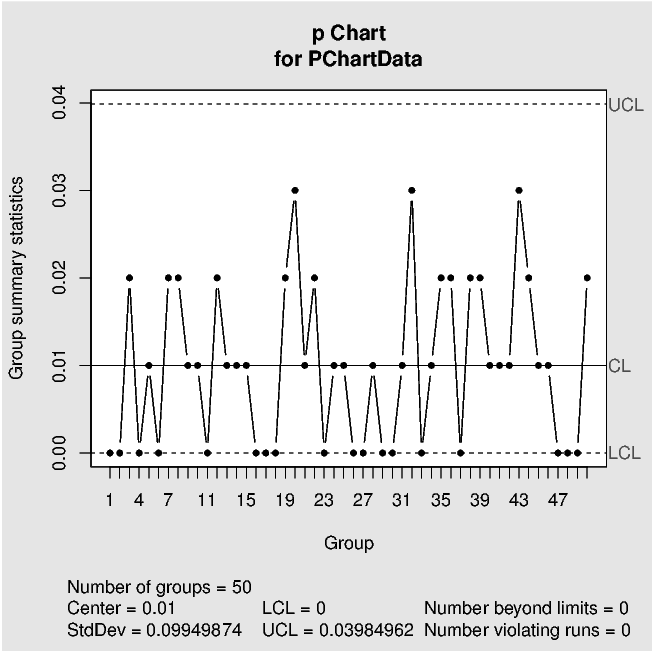
\includegraphics[width=0.7\linewidth]{p-charts}
\caption{}
\label{fig:p-charts}
\end{figure}

\end{frame}
%==================================================================== %
\begin{frame}
	\frametitle{p-Charts}
	\Large

Note that observations of proportion nonconforming below a positive lower control limit are cause for concern as they are more frequently evidence of improperly calibrated test and inspection equipment or inadequately trained inspectors than of sustained quality improvement.

\end{frame}
%==================================================================== %
\begin{frame}
	\frametitle{p-Charts}
	\Large
\begin{itemize}
\item Some organizations may elect to provide a standard value for p, effectively making it a target value for the proportion nonconforming. \item This may be useful when simple process adjustments can consistently move the process mean, but in general, this makes it more challenging to judge whether a process is fully out of control or merely off-target (but otherwise in control).
\end{itemize}


\end{frame}
%==================================================================== %
\begin{frame}
	\frametitle{p-Charts}
	\Large
\noindent \textbf{Potential pitfalls}\\
There are two circumstances that merit special attention:
\begin{itemize}
\item Ensuring enough observations are taken for each sample
\item Accounting for differences in the number of observations from sample to sample
\end{itemize}


\end{frame}
%==================================================================== %
\end{document}